\documentclass[a5paper]{article}
\usepackage[a5paper, top=8mm, bottom=8mm, left=8mm, right=8mm]{geometry}

\usepackage{polyglossia}
\setdefaultlanguage[babelshorthands=true]{russian}

\usepackage{fontspec}
\setmainfont{FreeSerif}
\newfontfamily{\russianfonttt}[Scale=0.7]{DejaVuSansMono}

\usepackage[font=scriptsize]{caption}

\usepackage{amsmath}
\usepackage{amssymb,amsfonts,textcomp}
\usepackage{color}
\usepackage{array}
\usepackage{hhline}
\usepackage{cite}

\usepackage[hang,multiple]{footmisc}
\renewcommand{\footnotelayout}{\raggedright}

\PassOptionsToPackage{hyphens}{url}\usepackage[xetex,linktocpage=true,plainpages=false,pdfpagelabels=false]{hyperref}
\hypersetup{colorlinks=true, linkcolor=blue, citecolor=blue, filecolor=blue, urlcolor=blue, pdftitle=1, pdfauthor=, pdfsubject=, pdfkeywords=}

\usepackage{tabu}

\usepackage{graphicx}
\usepackage{indentfirst}
\usepackage{multirow}
\usepackage{subfig}
\usepackage{footnote}
\usepackage{minted}

\sloppy
\pagestyle{plain}

\title{Domain-Driven Design}
\author{Юрий Литвинов\\\small{yurii.litvinov@gmail.com}}

\date{13.04.2018г}

\begin{document}

\maketitle
\thispagestyle{empty}

\section{Введение}

В этой лекции будет продолжение рассказа про Domamin-Driven Design, а конкретно, про ``тактические'' его аспекты --- идеи и паттерны, близкие к реализации.

Про Domain-Driven Design немного говорилось в прошлый раз, напомню основные моменты:

\begin{itemize}
    \item Domain-Driven Design (или предметно-ориентированное проектирование) --- популярная методология проектирования ПО, которая основана на анализе предметной области и реализации модели предметной области в приложении. Архитектуру в рамках этой методологии предлагается строить не исходя из сиюминутных потребностей реализации, а вокруг ``смыслового ядра'', которое отражает основные сущности реального мира, с которым будет работать программа (или семейство программ).
    \item Модель предметной области выражается прежде всего в коде --- сущности предметной области становятся классами языка программирования, используемого для реализации. Также для обсуждения предметной области с экспертами, а также для документирования модели, часто используются диаграммы.
    \item Немаловажную роль как в создании модели, так и в её ``фиксации'' и улучшении играет ещё и устное общение. Неудачные названия классов или методов, неуклюжие и непонятные описания взаимодействий прекрасно слышны в разговоре и являются поводом для того, чтобы посмотреть на модель ещё раз. Сам естественный язык часто подсказывает правильные архитектурные решения --- что неудивительно, язык сотни лет оттачивался как раз для того, для чего он нужен в DDD --- для передачи сути понятий. Ещё раз напомню, что архитектура --- это больше про понимание программы человеком, а не понимание программы компьютером, так что всякие гуманитарные вещи могут сильно помочь при разработке архитектуры.
    \item Модель определяет единый язык, на котором должны общаться все члены команды и эксперты предметной области, которые им помогают. Если какой-то термин зафиксирован как имя класса, использование его синонимов ни в диалогах, ни в документации, ни тем более в коде не допускаются, можно использовать только имя класса. Так же и с методами --- если действию дали название, можно использовать только его, и если это не удобно, название меняют. Это, во-первых, упрощает общение и сопровождение программы, во-вторых, способствует улучшению модели, постоянно её тестируя на предмет неконсистентностей, недопониманий и неоднозначностей.
    \item Модель появляется не только благодаря применению единого языка и последовательного именования всех нужных сущностей, она также ``выкристаллизовывается'' в процессе непрерывного рефакторинга и уточнения. Поскольку программисты редко владеют предметной областью, в которой они решают задачу, построить правильную и хорошую модель предметной области невозможно просто потому, что знаний не хватает. Есть понятие ``переработка знаний'' --- когда программисты строят модель, одновременно активно изучая предметную область. Узнав что-то новое, они включают это в модель, рисуют диаграммы, обсуждают их с экспертами, корректируют модель, и т.д. до тех пор, пока не будет достигнуто достаточное понимание. Цель ``переработки знаний'' --- не получить понимание, достаточное для реализации программы, а понять принципы, по которым работает сама предметная область, а уже потом написать программу. Интересно, что если модель хороша и программисты неплохи в выделении абстракций, то в процессе переработки знаний кое-чему научиться могут и эксперты.
\end{itemize}

Дальнейший рассказ является, по сути, кратким пересказом книги Эрик Эванс, ``Предметно-ориентированное проектирование. Структуризация сложных программных систем''. М., ``Вильямс'', 2010, 448 стр., по крайней мере, первых трёх её частей. Если есть время, лучше её прочитать, если нет, то по этому конспекту, я надеюсь, можно составить общее представление. Некоторые примеры и все картинки взяты оттуда.

\section{Единый язык}

Единый язык --- одно из ключевых понятий предметно-ориентированного проектирования. Необходимость его введения связана с тем, что программисты и специалисты предметной области разговаривают на разных профессиональных жаргонах и изначально не понимают друг друга. Если программисты будут общаться в терминах реализации, экспертам это будет не очень полезно. Причём, что особенно опасно, непонимание будет, скорее всего, скрытым --- они будут чувствовать себя, как типичные студенты на лекции по матанализу: вроде общий смысл улавливается, но местами происходит что-то такое, с чем, кажется, можно будет разобраться потом, прочитав конспект. Но лекцию по матанализу ведёт человек, разбирающийся в предмете, а обсуждающий с заказчиком программу программист, возможно, просто неправ, или подсознательно маскирует своё собственное непонимание техническими терминами, отчего и эксперт его не понимает, но не может поправить.

На самом деле, даже среди разработчиков одной группы вырабатывается свой жаргон, который может быть непонятен новичкам и даже опытным членам соседних групп, работающих над тем же проектом. Это плохо, во-первых, тем, что необходимость постоянно переводить понятия с одного языка на другой вызывает ``размытие'' этих понятий и некоторую неопределённость, причём, каждый может делать перевод по-своему, что усиливает хаос. Во-вторых, это плохо тем, что один термин может использоваться в разных (иногда очень слегка разных) значениях --- внутри проекта возникают ``ереси'', что приводит уже к откровенной путанице и багам в коде.

Поэтому предметно-ориентированное проектирование предписывает выработку единого языка и использование его повсюду в проекте, от составления технического задания до имён методов, переменных и тестов. В единый язык входят термины предметной области --- как правило, они становятся именами классов, отношения между понятиями и действия, которые сущности могут выполнять --- это имена методов, также в язык попадают имена паттернов, используемых при проектировании системы, даже если их в предметной области нет (например, ``репозиторий'' или ``спецификация''). Ещё единый язык должен содержать понятия, относящиеся к высокоуровневой архитектуре системы, которые напрямую невыразимы в коде --- уровни, ограничения на взаимодействие (например, понятие ``канал'' в архитектурном стиле ``каналы и фильтры'' может явно в коде никак не выражаться, но в архитектуре играет ключевую роль).

Единый язык не создаётся мгновенно, он эволюционирует вместе с пониманием предметной области, моделью и кодом, который эту модель реализует. Поэтому за изменениями языка, которые возникают естественно в разговорах (а помним, что общаться можно только на едином языке), надо следить и соответственно рефакторить модель или код. Например, если все начали говорить ``связь'' вместо ``ассоциация'' (потому что так короче и благозвучнее), надо переименовать соответствующий класс и в коде.

На самом деле единых языков в проекте может быть много, как бы бредово это ни звучало. Если проект состоит из нескольких более-менее обособленных частей, то почему нет, каждая из них может иметь свой язык. Например, система планирования грузоперевозок вполне может использовать библиотеку алгоритмов на графах, в самой системе связь может называться ``перевозка'', а в библиотеке --- ``ребро''. Если есть чёткая граница между сферами действия разных языков (и разных моделей и даже мировоззрений, которые связаны с языком) и определены правила преобразования одного в другое (выражающиеся в коде в виде фасадов и адаптеров), то почему нет, это помогает уменьшить общую сложность системы. Если чёткой границы нет и модели (и языки) начинают проникать друг в друга, возникает путаница, которая может привести к провалу проекта.

Небольшой пример важности единого языка. Положим, нам надо сделать систему планирования грузоперевозок и мы рассматриваем задачу прокладки маршрута перевозки через какой-то пункт таможенного контроля. Мы везём груз из точки А в точку Б через 0 или больше пунктов таможни, и у нас есть планирвощик маршрута, которому можно сказать точки А, Б и таможни, чтобы он выдал расписание перевозки. Модель глазами программиста могла бы выглядеть так:

\begin{center}
    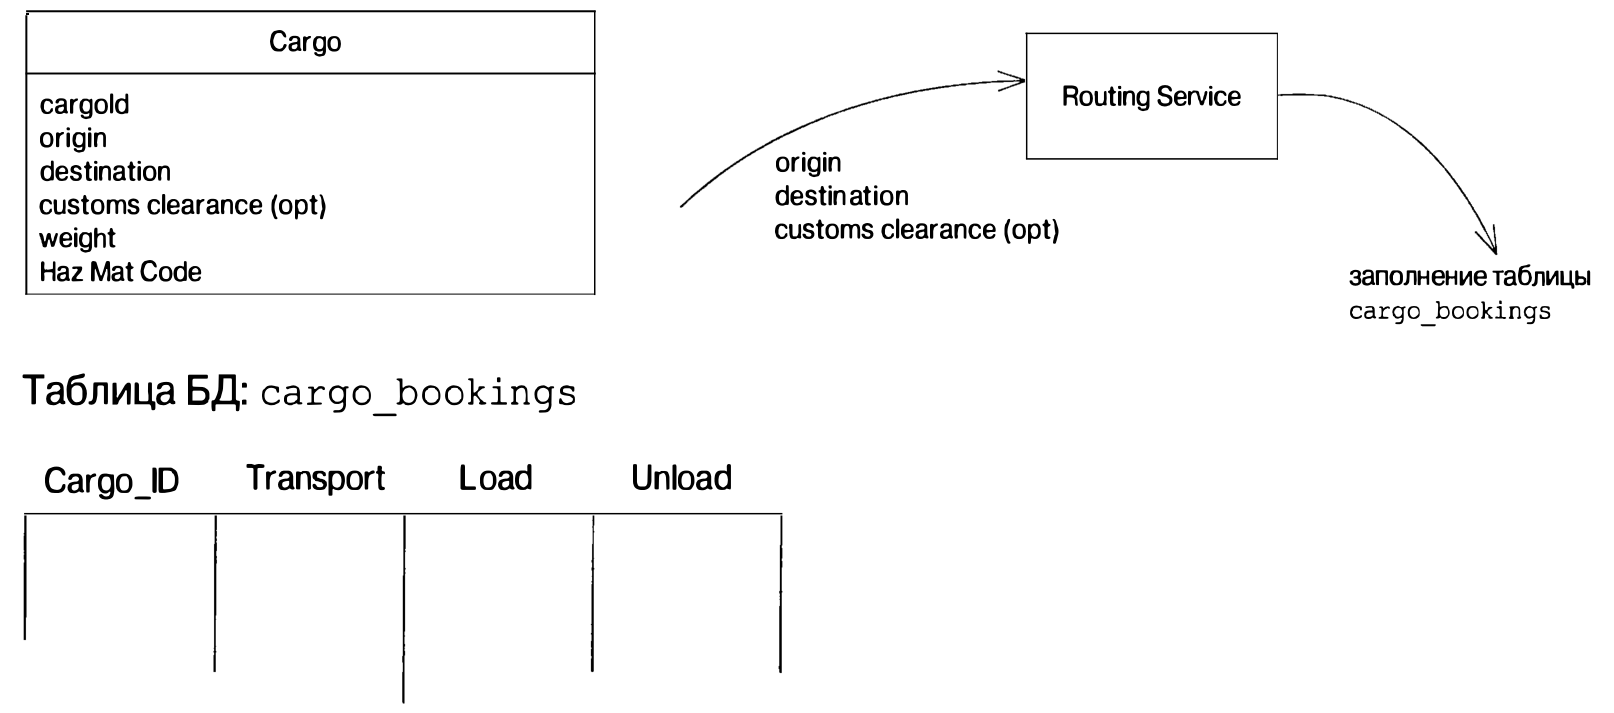
\includegraphics[width=0.9\textwidth]{lowAbstractionLanguage.png}
\end{center}

Представьте себе обсуждение с экспертом по логистике вопроса изменения пункта растомаживания:

\textit{``Тогда мы удаляем все строки в таблице отправки грузов с задан­ным идентификатором груза, потом передаем пункт отправки, пункт назначения и новый пункт растаможивания в Маршрутизатор (Routing Service) и он заполняет таблицу заново. В объект Груз (Cargo) надо добавить логический переключатель, указывающий, есть ли данные в таблице отправки.''}

Сравним это с вот такой моделью:

\begin{center}
    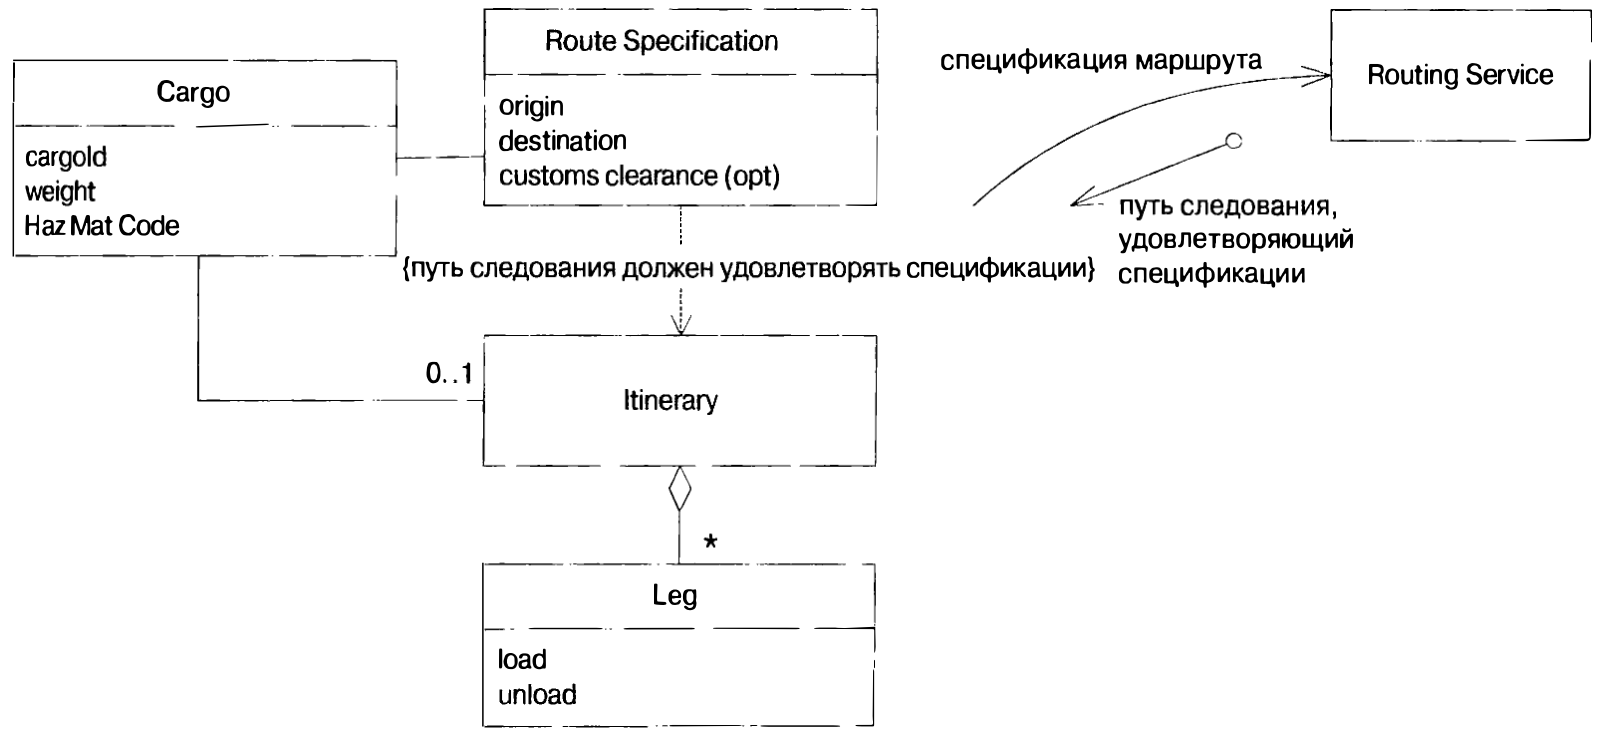
\includegraphics[width=0.9\textwidth]{highAbstractionLanguage.png}
\end{center}

Тут наше обсуждение могло бы выглядеть так:

\textit{``При изменении любого из атрибутов в Спецификации маршрута (Route Specification) мы удаляем старый Маршрут (Route) и просим Маршрутизатор (Routing Service) построить новый маршрут на основе новой Спецификации маршрута.''}

Получилось короче, более точно и даже более полно, потому что в модели выше надо было ещё пояснять, когда сбрасывать маршрут, а тут появилось понятие ``Спецификация маршрута''. Вторая модель (и язык, с ней связанный) по сути радикально систему не меняет (Leg и Itinerary всё также могут быть таблицами в БД), оставляет гораздо меньше возможностей для взаимного непонимания и ошибок, с ним связанных.

Ещё один хороший пример использования единого языка, из книжки:

\begin{center}
    \textit{Если передать в \textbf{Маршрутизатор} пункт отправки, пункт назначения, время прибытия, то он найдет нужные остановки в пути следования груза, а потом, ну... запишет их в базу данных.}

    \vspace{4mm}

    \textit{Пункт отправки, пункт назначения и все такое... все это идет в \textbf{Маршрутизатор}, а оттуда получаем \textbf{Маршрут}, в котором записано все, что нужно.}

    \vspace{4mm}

    \textit{\textbf{Маршрутизатор} находит \textbf{Маршрут}, удовлетворяющий \textbf{Спецификации маршрута}.}
\end{center}

Опять-таки, видно, что хорошая модель позволяет строить фразы коротко, точно и без технических подробностей. Но тут ещё видно, как естественный язык помогает процессу разработки архитектуры --- мы начали с первой фразы, запнулись, потому что у нас не было сущности ``Маршрут'', добавили её в модель, стало лучше, но теперь нам не нравится ``и всё такое'', что мы побеждаем добавлением понятия ``Спецификация маршрута''. Конечно, натуральный язык и метафоры могут завести не туда, но если это случится, то это скорее проблемы понимания предметной области, и их будет проще найти, чем если бы эти проблемы были бы спрятаны в таблицах в базе данных.

\section{Модель и реализация}

Модель предметной области полезна только в том случае, если она непосредственно связана с кодом. Бывает так, что люди, вообразившие себя крутыми архитекторами, рисуют огромную модель предметной области в виде диаграммы классов UML, которую невозможно эффективно реализовать, например, положить в базу данных. Тогда обычно разработчикам приходится частично игнорировать модель, решая свои чисто практические задачи. Это приводит к тому, что код и модель расходятся, при этом модель становится даже вредна, поскольку врёт об устройстве кода.

Бывает и наоборот, люди, вообразившие себя крутыми agile-developer-ами, начинают ``фигачить код'' безо всякой архитектуры-шмархитектуры. В результате получается программа, полученая хаотичным наслоением слабо связанной функциональности, которую тяжело читать, сопровождать, добавлять новую функциональность. Эванс в книжке кратко описывает два таких проекта и делает интересное наблюдение, что результаты получились примерно одинаковыми.

Из этого следует вывод, что модель всегда должна быть связана с кодом, а добиться этого можно только если каждый архитектор пишет код и любой программист участвует в моделировании. Практика, принятая в некоторых enterprise-проектах, когда аналитики сначала строят модель предметной области, а затем программисты её реализуют, пагубна именно поэтому --- модель может игнорировать особенности реализации, а знания аналитиков не будут полностью переданы программистам. И наоборот, новые интересные знания могут быть получены при попытке выразить модель в коде, эти знания аналитикам (или архитекторам) не попадут. В результате программистам придётся проделывать работу по анализу предметной области фактически заново, и ``prescriptive architecture'' разойдётся с ``descriptive architecture''. Есть даже хороший термин ``разрушительный рефакторинг'', когда программисты, не понимая глубоко предметную область, рефакторят программу так, чтобы было удобно реализовывать требуемую функциональность. В этот момент, скорее всего, потеряется самая суть программы, её смысловое ядро, и это будет просто работающее приложение, которое будет делать что нужно. DDD же ставит своей целью создавать системы, которые делают больше и лучше, чем нужно (при этом будучи менее трудозатратными при разработке).

Поэтому модели в DDD приходится быть одновременно и моделью анализа, и моделью проектирования. Мы с её помощью пытаемся понять предметную область, и она же используется для того, чтобы писать код (причём, одновременно). Так что если модель окажется полной технических деталей, то анализ предметной области и общение с экспертами неизбежно пострадают, а если она будет слишком абстрактной или непроработанной, то пострадает реализация. Необходим баланс, который достигается обычно за несколько итераций --- описываем предметную область, пытаемся её реализовать, получается плохо, правим модель и рефакторим код, пытаемся описать предметную область в новой модели, получается неуклюже, снова рефакторим модель и т.д., пока не придём к модели, которая хорошо служит и коду, и объяснению предметной области. 

При этом, разумеется, необходимо, чтобы выбранный язык программирования поддерживал парадигму моделирования --- например, с ООП всё довольно легко, а вот с чисто структурными языками, например, C, может быть плохо --- в них не выразить естественным образом сущности с состоянием и поведением, свойственные реальному миру. А вот Prolog, напротив, хорош, он близок исчислению предикатов, так что если мы можем построить модель в терминах фактов и правил вывода, на Прологе программа запишется очень естественно.

Ещё не рекомендуется разделять модель, которая служит основой реализации, и модель, которую показывают пользоателю. Пример --- в Internet Explorer закладки хранились как файлы-ярлыки на диске, но пользователю про это ничего не говорилось. Хочет пользователь сохранить закладку с символом ``:'', а ему ошибка --- неправильное имя файла. И пользователь не может понять, какого к чёрту файла, он просто закладку сохранил. А вот если бы закладки и показывались как файлы, то пользователь мог бы сортировать их с помощью файлового менеджера или вообще скрипта, и был бы более счастлив.

\section{Изоляция предметной области}

Хорошо, допустим, мы смогли построить модель предметной области. Но этого недостаточно, чтобы получить работающую программу --- нужен ещё пользовательский интерфейс, сеть, база данных, всякого рода вспомогательный код, логирование, обработка ошибок, юнит-тесты и т.д. Основная идея DDD в том, что всё это должно быть архитектурно отделено от модели предметной области, чтобы код модели --- код, в котором сосредоточена вся суть приложения --- мог быть максимально простым, небольшим по размеру и содержащим только существенные для смысла системы вещи. Всё остальное должно находиться в отдельных модулях и просто использовать классы доменной модели.

Самый популярный способ достижения такого разделения (хотя и не единственный) --- уровневая архитектура. Программа реализуется в виде набора уровней, где каждый уровень может непосредственно взаимодействовать только с уровнями ниже. Способов разделения на уровни бывает много (трёхзвенная архитектура, семь уровней OSI, четыре уровня TCP/IP и т.д.), DDD требует лишь, чтобы среди всех уровней был уровень предметной области, на котором и сосредоточены все классы модели.

Довольно типичный для информационных систем способ разделения на уровни представлен на картинке:

\begin{center}
    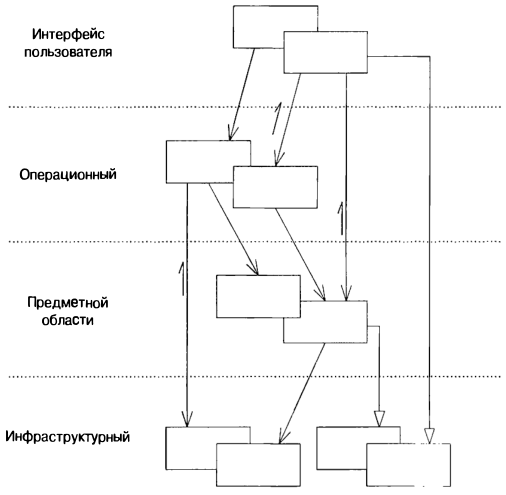
\includegraphics[width=0.6\textwidth]{layers.png}
\end{center}

Уровень интерфейса отвечает только за взаимодействие с пользователем и реализует только отображение и обработку событий. Никакой содержательной логики в нём быть не должно. Операционный уровень (application layer) занимается координацией действий бизнес-объектов, которые находятся на уровне предметной области. Операционный уровень тоже должен быть очень простым, его ответственность --- это инициализировать систему и по сигналу от интерфейса инициировать нужные пользователю операции. Инфраструктурный уровень содержит все вспомогательные вещи, неспецифичные для данной предметной области, например, код работы с базой данных или код работы с сетью.

Уровень предметной области содержит бизнес-объекты, которые ничего интересного кроме, собственно, реализации бизнес-правил, не делают. Их реализация должна быть максимально простой, и именно их реализации следует уделять максимум внимания, потому как именно уровень предметной области определяет конкурентные преимущества и полезность программы.

Операционный уровень специфичен для каждого конкретного приложения, тогда как уровень предметной области может разделяться между несколькими приложениями в семействе. На операционном уровне из классов уровня предметной области собирается то, что делает конкретно наше приложение, операционный уровнь же координирует бизнес-объекты. Но бизнес-регламенты (например, последовательность действий в бизнес-процессе) должны быть реализованы на уровне предметной области, потому как они хоть и координируют действия других объектов, но объективно присутствуют в предметной области и могут быть переиспользованы в других приложениях. Операционному уровню также запрещается иметь состояние (кроме, быть может, состояния, необходимого для общения с пользователем приложения, типа прогресса операций).

Инфраструктурный уровень поддерживает все уровни выше. Он может обеспечивать архитектурную среду для всех остальных уровней (например, Java Beans или ROS), может содержать специфичный для приложения код работы с третьесторонними библиотеками и технологиями (например, Object-Relational Mapping). Может показаться противоестественным, что базовые классы для уровней выше могут быть на инфраструктурном уровне (то есть деревья наследования растут вверх), но если подумать, кто о ком больше знает --- предок или потомок, то становится понятно, что концептуально всё ок.

Уровням ниже, естественно, иногда требуется общаться с уровнями выше. Даже инфраструктурный уровень, если он не состоит только из библиотек, может инициировать действия на уровнях выше (например, получение сетевого пакета вызывает обработку на операционном уровне). Поскольку общаться напрямую уровни не могут, применяются приёмы ``косвенного'' вызова --- callback-и (или виртуальные методы --- hook-и), паттеррн ``Наблюдатель'', ``дедушка всех паттернов'' MVC. Такой подход несколько затрудняет отладку, но позволяет разрабатывать каждый уровень независимо, и не думать, как будут пользоваться кодом уровня другие.

В реальной жизни часто встречается диаметральная противоположность такого подхода --- антипаттерн ``умный GUI''. Это когда вся бизнес-логика приложения реализуется прямо в классах, отвечающих за пользовательский интерфейс, как правило, в обработчиках библиотечных событий. При этом даже работа с БД может выполняться из кода GUI.

Как ни странно, это не всегда плохо. Во-первых, есть куча тулов для быстрой разработки пользовательских интерфейсов, при этом подходе их можно задействовать на полную --- большая часть приложения будет просто сгенерена. Во-вторых, это быстро --- рабочее приложение таким способом можно написать за пару часов, при этом нет оверхеда на создание классов, интерфейсов, наладку общеиня между уровнями, организацию взаимодействия. Легко добавлять в приложение новые фичи --- просто кидаем на форму новый контрол, цепляем к нему новый обработчик, и в продакшн. Причём, поскольку код каждого куска такой функциональности довольно прост, его несложно поддерживать или переписать заново.

Однако если ожидаемый размер проекта превышает где-то 3000 строк кода, ``Умный GUI'' быстро становится антипаттерном. Почему: невозможно проектирование по модели, классов предметной области просто нет, есть методы-обработчики, в которых код интерфейса смешан с бизнес-правилами и инфраструктурным кодом. Поэтому переиспользование бизнес-правил чрезвычайно затруднено, фактически, если две фичи требуют одного бизнес-правила, его надо реализовать дважды. Сложное поведение в такой ситуации оказывается сложно реализовать --- не получится аккуратно декомпозировать его на набор взаимодействующих объектов без разделения на уровни. Практически невозможна интеграция с другими системами --- всё завязано на GUI, так что реализовать отдельный API для интеграции может быть очень сложно (опять-таки, в процессе сами собой появятся бизнес-объекты и уровни, так почему не сделать сразу нормально?).

\section{Основные структурные элементы модели}

В программе модель реализуется с помощью различных ``элементарных'' блоков, и не всегда тривиально. В первую очередь, следует подумать над ассоциациями. Если в предметной области одно из направлений ассоциации более приоритетно, чем другое (например, ``страна -- президент'', скорее всего, предполагает доступ от страны к президенту), то имеет смысл сделать ассоциацию однонаправленной. В идеале все или почти все ассициации должны быть однонаправленными, потому что двунаправленная ассоциация делает невозможным понять один объект в отрыве от другого. Также следует по возможности минимизировать множественность (возможно, добавив квалификаторы, типа ``страна -- год -- президент'') и минимизировать количество ассоциаций вообще. Меньше связей --- проще анализ и сопровождение.

Следующая задача --- решить, кто в модели будет сущностью, а кто --- объектом-значением. Сущность имеет собственную идентичность, не зависящую от её состояния, тогда как объект-значение определяется только значениями своих атрибутов. Это всё очень похоже на ссылочные типы и типы-значения в языках программирования, но в реальной жизни всё гораздо сложнее, потому как ссылочная идентичность не переживает сериализации. Кроме того, одна и та же сущность может вообще представляться несколькими совершенно разными объектами (например, когда ввод данных в систему происходит в нескольких приложениях), или существовать в нескольких экземплярах в системе (например, в случае с распределёнными транзакциями). Тем не менее, система в любом случае должна корректно устанавливать идентичность сущности. Простой пример возможных проблем --- входящий звонок от клиента. Это может быть старый клиент звонящий с известного нам номера, либо старый клиент, который поменял себе номер (и мы всё равно должны как-то догадаться, что уже имели с ним дело), или даже новый клиент, которому почему-то достался номер старого клиента (и мы должны догадаться, что это новый клиент).

В реальной жизни естественные механизмы обеспечения идентичности не очень-то существуют. Людей, например, можно было бы идентифицировать по номеру паспорта, но паспорта меняют. Можно было бы по ИНН, но не у всех он есть. Можно было бы по СНИЛС, но он тоже есть не у всех. Имя и фамилия тем более не лучший способ идентификации, потому как даже я учился на одном потоке с человеком, у которого полностью совпадали со мной имя, фамилия и первая буква отчества (и год рождения, раз мы были на одном потоке). И нас правда часто путают до сих пор, меня уже несколько раз приглашали работать Java-программистом (один раз в Яндекс). Эрик Эванс в своей книге рассказывал гораздо более грустную, но аналогичную историю.

Часто в качестве идентификатора используют некий суррогатный атрибут, например, GUID, назначаемый объекту при создании. Иногда этот атрибут даже становится доступен пользователю (например, трек-номер почтового отправления), иногда нет (например, у каждого документа в Google Docs есть уникальный Id, который нигде в интерфейсе не показан, поэтому в одной папке вполне может быть два документа с одним именем). Иногда есть естественный атрибут, однозначно идентифицирующий сущность, например, номер кресла в кинотеатре. Да, кресло могут переставить на другое место или сменить нумерацию, но для информационной системы кинотеатра важна не физическая идентичность кресла, а место, билет на которое можно продать. Естественные атрибуты лучше суррогатных, поскольку сами собой решают проблему идентификации ``дубликатов'' объекта (той же сущности, но из другой системы), но пользоваться ими надо очень осторожно, потому что то, что вам кажется уникальным и присущим всем объектам свойством, на деле может оказаться не так.

От способа идентификации требуется, чтобы он переживал сохранение, загрузку, передачу в другую систему и представление там в другом формате. Соответственно, нужна операция идентификации, которая по двум данным объектам может сказать, один и тот же это объект или нет. Ссылочное равенство, очевидно, не подходит для большинства практически полезных случаев, поэтому способ идентификации на самом деле важное архитектурное решение.

Можно всё в системе сделать сущностями, но тогдда все рассуждения про сложные правила идентификации, приведённые выше, оказываются применимы к вообще каждому объекту системы, что, во-первых, доставит боль при реализации, а во-вторых, повредит эффективности. Поэтому всё, что можно, лучше превращать в объекты-значения. Объекты-значения должны быть единым концептуальным целым (например, имя и фамилия --- это не два атрибута сущности ``Человек'', а один объект-значение, описывающий человека), очень желательно делать их немутабельными. Объекты-значения вполне могут ссылаться на сущности, и наоборот, сущности могут ссылаться на объекты-значения. Обратите внимание, что объекты-значения может быть вполне валидно реализовывать как ссылочные типы (например, чтобы обеспечить разделяемость). Немутабельность, кстати, полезна не только для обеспечения разделяемости, а ещё и для того, чтобы иметь возможность возвращать или передавать как параметр объект-значение --- мы отдаём его вовне, но точно знаем, что его никто не сломает. Разделяемость, кстати, хоть и хороша в плане экономии памяти и места в базе данных, может быть плоха, если система распределённая --- при каждом обращении к разделяемому объекту придётся делать сетевой запрос.

Обратите внимание, что сущность объект или значение --- это не его врождённое свойство, а вопрос проектирования конкретной системы. Один и тот же объект может играть роль как сущности, так и значения, даже в рамках одной предметной области. Например, бывают билеты на места с указанием места (и тогда каждое место --- сущность, у него есть идентичность, исключающая возможность продать два билета на одно место), а бывают билеты без указания места (и тогда важно только количество мест, оно будет объектом-значением). В последнем случае считать место сущностью будет даже неправильным (хоть на месте всё ещё написан его номер), поскольку в разы без всякой нужды усложняет систему.

В DDD разрешено и даже поощряется то, что считается дурным тоном в ООП --- классы без состояния, фактически представляющие собой набор статических методов. В DDD их называют ``службами''. В службы выносится код, который не имеет естественного места в ``настоящих объектах'' --- часто это операция, выполняемая над объектами нескольких разных классов, где все объекты равноправны, поэтому нельзя естественным образом поместить эту операцию в один из классов-участников --- например, различного рода диспетчеры или менеджеры. Службам, как правило, запрещается иметь состояние, так что вызывать методы службы можно отовсюду и в любом порядке, не заботясь о порядке вызовов.

Последней элементарной частью модели является модуль. Да, это модули в обычном для языков программирования смысле, DDD лишь призывает использовать их не как техничческое средство группировки классов, а как реальный механизм декомпозиции предметной области. Классы следует объединять в модули не по принципу высокой внутренней связности (cohesion) и низкой внешней зависимости (coupling), а семантически. Модуль --- это важная часть модели, модули должны быть определены так, чтобы повышать ``объясняющую способность'' модели предметной области. А высокая связность и низкая зависимость при этом получатся сами собой. Если это не так, имеет смысл порефакторить модель. Имена модулей должны естественным образом вписываться в единый язык модели.

\section{Цикл существования объекта модели}

Объекты в информационных системах часто обладают несколько более сложным жизненным циклом, чем ``создали, вызвав конструктор -> попользовались -> удалили''. Общий вид цикла существования объекта модели предметной области такой:

\begin{center}
    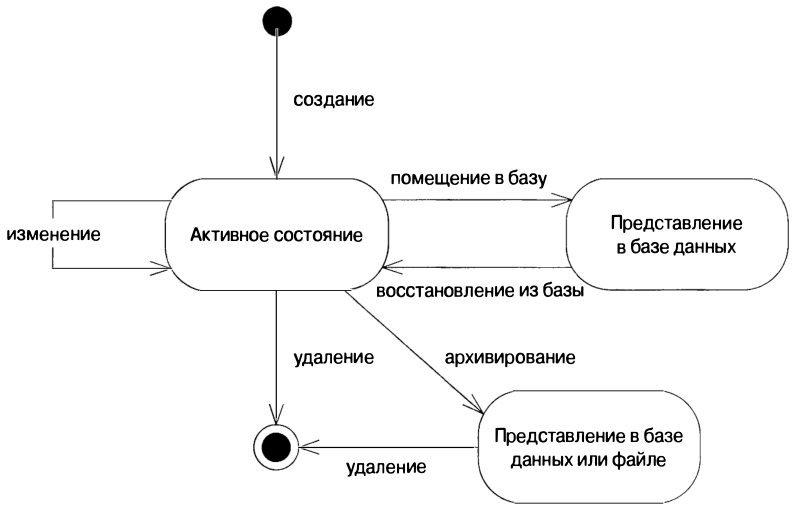
\includegraphics[width=0.8\textwidth]{objectLifeCycle.png}
\end{center}

Тут, как обычно, возникают проблемы с идентичностью объекта, если это сущность, а не значение, но кроме этого, добавляются проблемы с целостностью объекта и с излишней сложностью управления его состоянием. Для решения этих проблем применяются некоторые широко известные патерны проектирования.

Первый паттерн --- паттерн ``Агрегат''. Агрегат --- это изолированный кусок модели, имеющий ``корень'' и ``границу''. Доступ ко всем элементам агрегата возможен только через его корень. Корень представляет собой объект-сущность и имеет свою идентичность в рамках всего приложения. Остальные объекты в агрегате могут быть как сущностями, так и значениями, и они должны поддерживать свою идентичность только в рамках агрегата. Для чего это нужно --- для упрощения и декомпозиции модели. Когда мы пишем агрегат, мы можем думать только о взаимосвязи объектов внутри агрегата, а когда мы пишем код, пользующийся агрегатом, мы можем думать только о его корне. Так что агрегат --- это такая единица инкапсуляции программы. Как класс, только включает в себя, возможно, несколько классов. С технической точки зрения аккуратное разделение на агрегаты в разы облегчает обновления в базе данных: транзакции, затрагивающие разные агрегаты, гарантированно не мешают друг другу.

Содержимое агрегата на самом деле может быть видно снаружи, и не возбраняется отдавать ссылки на внутренние объекты агрегата, просто извне их нельзя хранить. Кроме того, у агрегата (как у класса) есть свои инварианты, и за поддержание их отвечает корень. Поэтому объекты, которые отдаются вовне, скорее всего, должны быть немутабельны, или быть копиями объектов внутри агрегата. Вот небольшой пример:

\begin{center}
    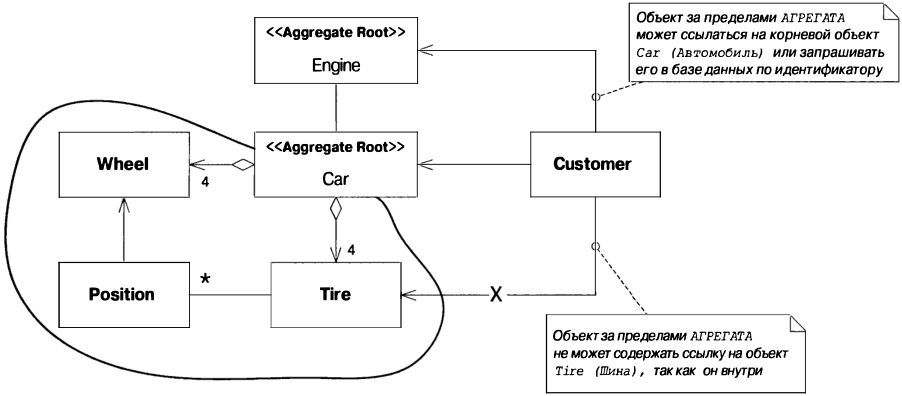
\includegraphics[width=0.9\textwidth]{aggregate.png}
\end{center}

Тут машина --- агрегат, содержащий в себе колёса и шины, поскольку пользователю может быть важно, на каком колесе какая шина, но глобально идентифицировать шины не требуется. Двигатель же наоборот, хоть и является неотъемлемой частью автомобиля, имеет собственный номер, так что уникален глобально (и на самом деле номер двигателя иногда проверяют безотносительно номера автомобиля). Автомобиль же предоставляет всю функциональность для управления шинами извне и поддерживает свои инварианты:

\begin{center}
    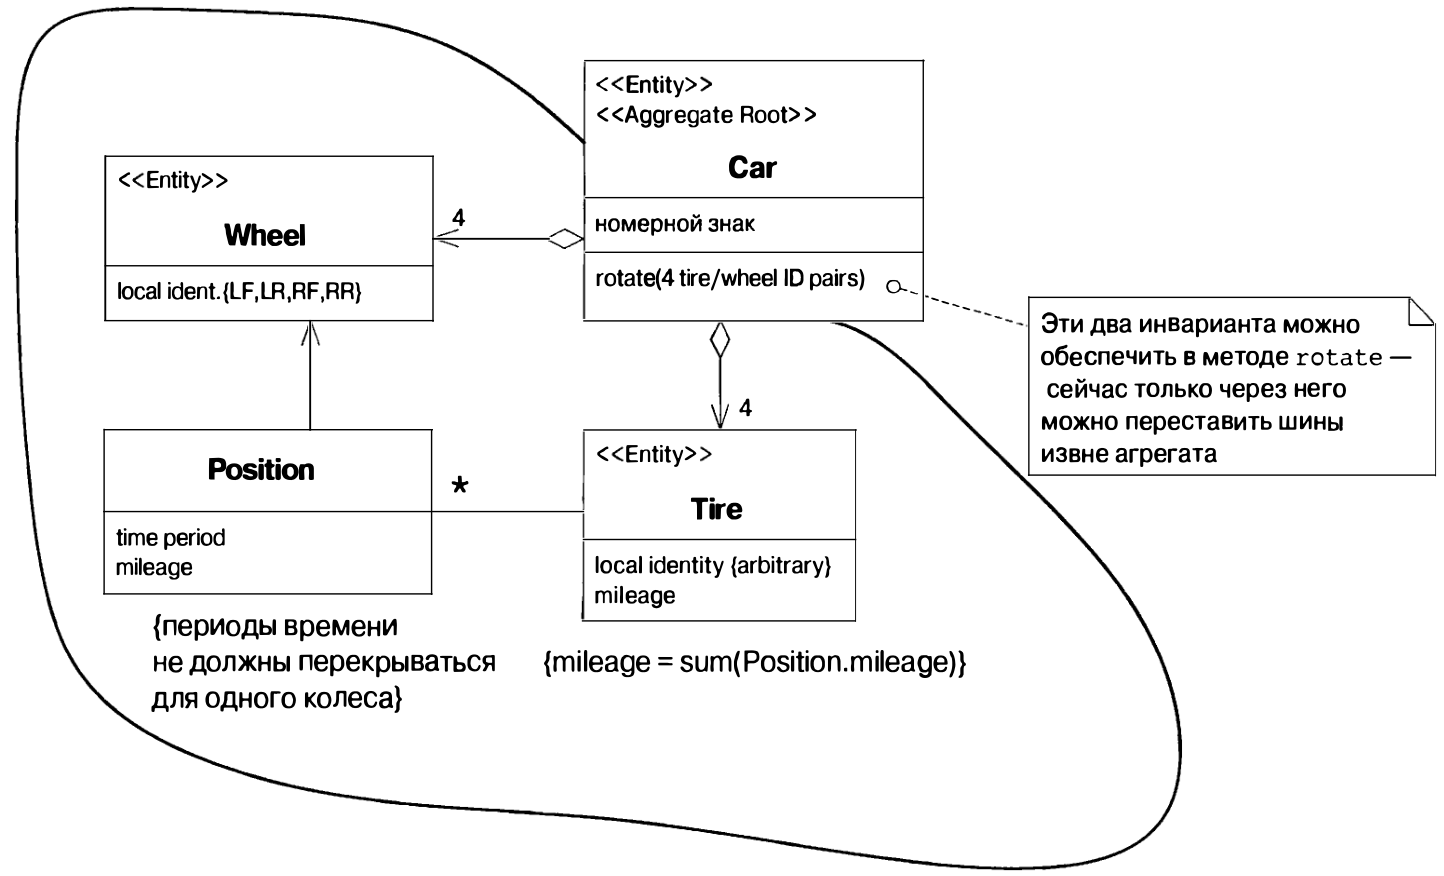
\includegraphics[width=0.9\textwidth]{aggregateInvariants.png}
\end{center}

Следующий паттерн --- ``Фабрика''. В DDD это несколько более архитектурный паттерн, чем похожий паттерн ``Абстрактная Фабрика'' Банды Четырёх, и на самом деле может использовать абстрактную фабрику для реализации. Задача фабрики --- создать и проинициализировать агрегат (или даже просто один объект) так, чтобы выполнялись его инварианты. Фабрика инкапсулирует сложную операцию создания объекта, не раскрывая его внутреннюю структуру, и при этом избавляет сам агрегат от необходимости уметь создавать себя. Фабрика вправе знать о структуре агрегата и манипулирвоать его внутренним содержимым непосредственно, а код извне --- нет, так что без фабрики пользоваться агрегатом было бы зачастую невозможно:

\begin{center}
    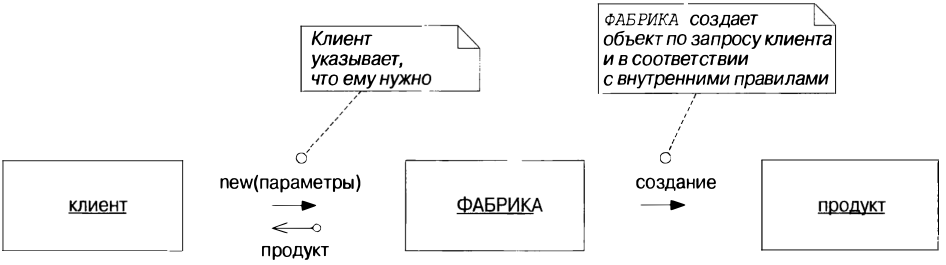
\includegraphics[width=0.9\textwidth]{factory.png}
\end{center}

Клиент передаёт фабрике параметры, указывающие, что ему нужно (может использоваться паттерн ``Спецификация'', о котором чуть потом), фабрика создаёт продукт и возвращает клиенту результат. Процесс создания атомарен в том смысле, что если что-то пошло не так, то клиент не получит результата вообще, как будто ничего не было. Для реализации фабрики могут использоваться паттерны ``Фабричный Метод'', ``Абстрактная Фабрика'', ``Builder''.

Интересно, что фабрики очень редко присутствуют явно в предметной области, тем не менее, являются важной частью модели и должны учитываться и в модели, и в едином языке на равных правах с ``настоящими'' объектами.

Фабрики могут использоваться не только для создания, но и для восстановления объекта из внешнего хранилища. В этом случае они не должны присваивать объекту новый идентификатор или вообще как-либо портить его идентичность. Вот пример такой фабрики, основная работа которой заключается даже не в создании объекта, а на самом деле в разборе XML-ки, куда был сохранён объект:

\begin{center}
    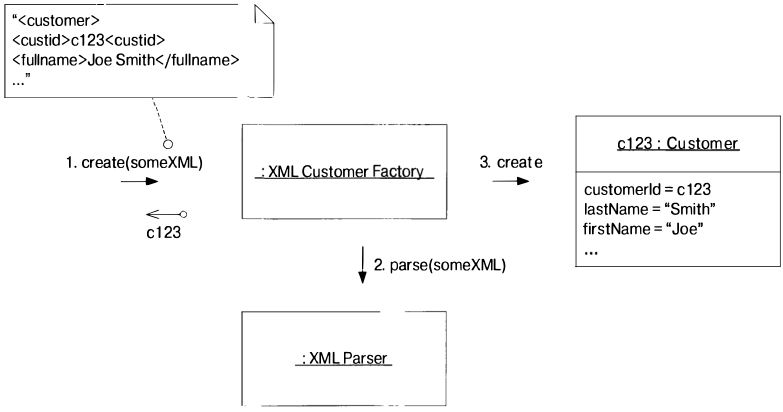
\includegraphics[width=0.9\textwidth]{xmlFactory.png}
\end{center}

Следующий паттерн управления жизненным циклом --- это ``Репозиторий'' (или ``Хранилище''). Репозиторий отвечает за хранение, сохранение и загрузку объектов при необходимости, предоставляя, как правило, глобальный доступ к объектам. Чаще всего репозиторий представляет собой прослойку между приложением и базой данных, при этом репозиторий сам может держать объекты в памяти и возвращать их по запросу. Нужно это для того, чтобы минимизировать количество переходов по ссылке с целью найти какой-либо объект, и вообще упростить задачу поиска. Представьте себе, что было бы, если бы все объеккты в программе можно было найти только переходом по ссылкам от некоторого корневого объекта. Если это CLI или задача в таком духе, где всё всегда помещается в память и данных очень немного, то всё было бы и так хорошо, но если большая часть данных всё время хранится в БД, то такой поиск блокировал бы половину базы, делая практически невозможной параллельную работу. Часто лучше хранить Id-шник нужного объекта и получать его при необходимости из репозитория, чем держать ссылку на объект.

Репозиторий может использовать развитый язык запросов, чтобы позволять клиенту найти объект. Часто это просто какой-то метод идентификации (типа суррогатного Id), но вполне может быть выборка объекта или коллекции объектов по их атрибутам или каким-то другим признакам (например, участии в отношениях с другими объектами). Опять-таки, может использоваться паттерн ``Спецификация'', про который чуть позже. Репозиторий за интерфейсом запросов прячет метод реального получения объекта: внутри он может использовать ORM-библиотеку + реляционную БД, может объектно-ориентированную БД, может (и часто использует) фабрики для создания объектов или восстановления объектов из базы. Задача репозитория --- делать так, чтобы обо всём этом не надо было заботиться клиентскому коду:

\begin{center}
    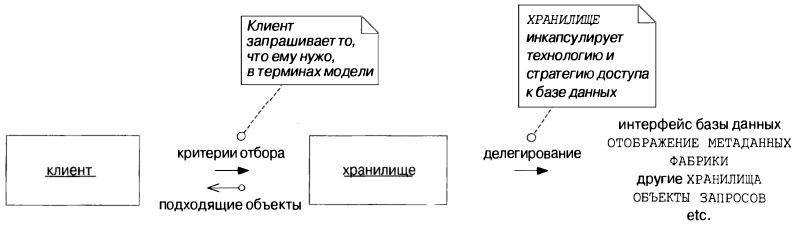
\includegraphics[width=0.9\textwidth]{repository.png}
\end{center}

Репозитории хорошо дружат с агрегатами, предоставляя доступ к корневому объекту агрегата по глобальному Id и собирая остальной агрегат при необходимости. 

\section{Пример, система грузоперевозок}

Рассмотрим большой пример, который с нуля попробуем спроектировать по принципам DDD и с использованием рассмотренных паттернов. Требуется разработать информационную систему для логистической компании, которая могла бы помогать принимать заказы на перевозку грузов, формировать маршрут перевозки и отслеживать движение груза по этому маршруту. Более подробно, вот первый набросок требований:

\begin{enumerate}
    \item Отслеживать ключевые манипуляции с грузом клиента
    \item Оформлять заказ заранее
    \item Автоматически высылать клиенту счет-фактуру по достижении грузом некоторого операционного пункта маршрута
\end{enumerate}

Первая задача при проектировании --- выделить сущности предметной области. Для этого требуется проинтервьюировать экспертов и узнать, что:

\begin{itemize}
    \item В работе с Грузом (Cargo) участвует несколько Клиентов (Customers), каждый из которых играет свою роль (Role)
    \item Должна задаваться (bе specified) цель (goal) доставки груза
    \item Цель (goal) доставки груза достигается в результате последовательности Переездов (Carrier Movement), которые удовлeтворяют Заданию (Specification)
\end{itemize}

Начинает вырисовываться единый язык, в котором пока только термины исключительно из предметной области. Нарисуем первое приближение модели в виде диаграммы классов UML:

\begin{center}
    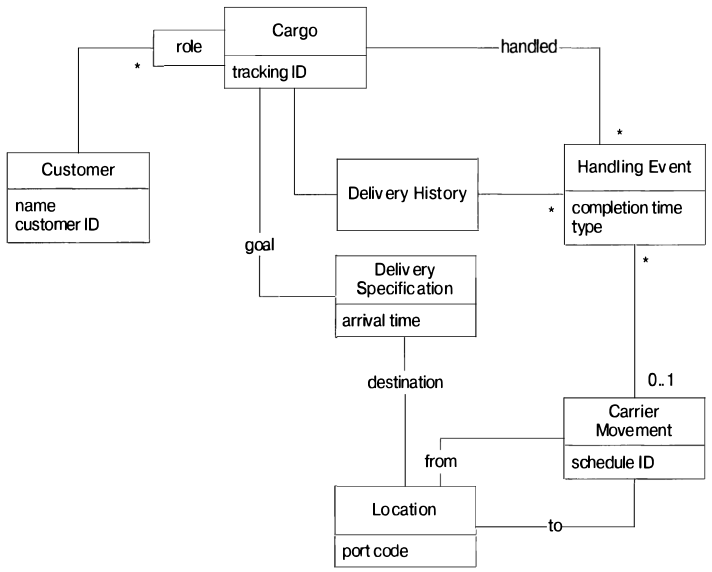
\includegraphics[width=0.7\textwidth]{cargoModel.png}
\end{center}

В центре системы находится Груз (Cargo), который нужно доставить в указанный порт не позднее указанного времени. Порт и время указываются в Delivery Specification, которой должен удовлетворять маршрут. Сама перевозка состоит из Handling Event-ов, связанных в Delivery History для каждого груза. Сам Handling Event имеет ссылку на соответствующий ему Carrier Movement, который, в свою очередь имеет место отправления и место прибытия. При этом есть ещё Customer, который может следить за своим грузом, имея его tracking ID. Обратим внимание, что Carrier Movement может за один раз перемещать сразу много грузов, что у Customer-а может быть много грузов, что Handling Event относится всегда к одному грузу, но в процессе доставки их, естественно, может быть много.

Какой-то набросок модели предметной области есть, дальше определимся с высокоуровневой структурой приложения. Будем использовать уровневую архитектуру (как это принято), с уровнем пользовательского интерфейса, операционным, предметной области и уровнем утилит. Операционный уровень (или уровень приложения) сейчас нам наиболее интересен, поскольку позволит определиться с требуемой функциональностью, а понимая её мы сможем целенаправленно уточнять модель. Судя по ТЗ и общему пониманию задачи, нам потребуются три разных приложения.

\begin{itemize}
    \item Мaршрутный запрос (Tracking Query) --- доступ к прошлым и нынешним манипуляциям с конкретным грузом, будет использоваться клиентом, чтобы следить за грузом.
    \item Служба резервирования (Booking Application) --- позволяет заказать доставку нового груза, будет использоваться клиентом.
    \item Служба регистрации событий (Incident Logging Application) --- регистрирует действия с грузом, будет использоваться сотрудниками логистической компании, чтобы вводить данные, которые потом будет показыввать Tracking Query.
\end{itemize}

Теперь можно заняться уточнением модели. Определимся, кто из объектов модели сущность, а кто может быть объектом-значением:

\begin{itemize}
    \item Клиент (Customer) --- сущность, у него точно есть идентичность;
    \item Груз (Cargo) --- сущность, тоже, идентичность следует из желания клиента знать, что с его грузом;
    \item Манипуляция (Handling Event) и Переезд (Carrier Movement) --- более сложно, но, в общем-то, в реальной жизни это уникальные операции, каждая из которых отличается от другой, и это важно для приложения, отслеживающего грузы --- значит, пусть будут сущностями;
    \item Местоположение (Location) --- сущность, нам надо различать два порта даже с одинаковым названием. Можно было бы использовать координаты, но это на самом деле не важно и не очень удобно, так что пусть будет сущность с искусственным механизмом идентификации (код порта);
    \item \textbf{История доставки (Delivery History)} --- сущность, локально идентичная в пределах агрегата ``Груз'' --- сама по себе история доставки уникальна и не взаимозаменяема с другими, но интересна только для конкретного груза;
    \item \textbf{Задание на доставку (Delivery Specification)} --- значение, потому как это просто задание, а не конкретная доставка. Его вполне можно переиспользовать, и два задания, требующие одного и того же --- по сути, одно задание.
    \item Всё остальное --- значения.
\end{itemize}

Теперь можно определиться с направленностью ассоциаций:

\begin{center}
    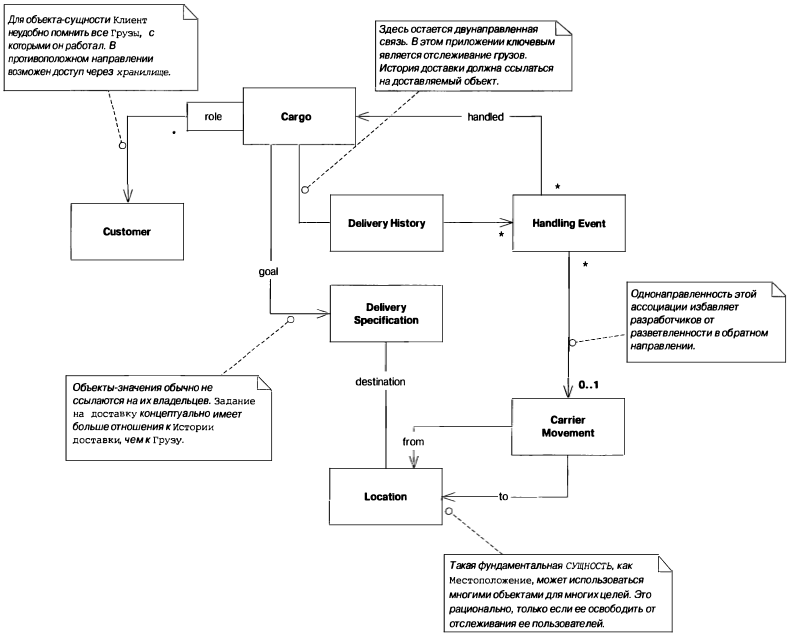
\includegraphics[width=0.7\textwidth]{cargoAssociations.png}
\end{center}

Мы постараемся минимизировать количество ссылок за счёт использования паттерна ``Хранилище''. Для начала разрешим Клиенту не ссылаться на Груз --- для постоянных клиентов,, которые отправляют тысячи грузов, держать их все в памяти неудобно, поэтому можно сделать Грузу ссылку на Клиент и в обратную сторону получать информацию с помощью запроса в БД, через ``Хранилище''. Дальше сделаем ассоциацию между Handling Event и Carrier Movement однонаправленной, от первого ко второму --- мы не хотим вести учёт грузовых кораблей, мы хотим вести учёт грузов, поэтому какие грузы везёт конкретный корабль --- не так важно, это можно узнать снова запросом к БД через репозиторий. Связи с участием Location должны быть все однонаправленными, причём в сторону Location, потому как местоположение используется много где и много кем, и ему вовсе не обязательно знать, кем именно. Между грузом и историей доставки связь всё-так будет двунаправленной, и будет циклическая зависимость между грузом, историей доставки и манипуляцией, но эта зависимость, судя по всему, присуща предметной области и от неё в модели особо никуда не деться. В реализации же можно заменить одну из ассоциаций на запрос к репозиторию.

Дальше определимся с агрегатами. Вокруг Груза есть некоторое количество локально идентичных объектов, поэтому естественно было бы сделать Груз корнем агрегата. А вот Handling Event, несмотря на то, что кажется логичным включить его в Груз, используется и сотрудниками логистической компании, чтобы отмечать статус груза, и тогда Handling Event надо уметь находить по Перевозке (приплыл корабль с сотней разных грузов --- надо все пометить как доставленные). Поэтому его разумно сделать корнем своего агрегата, не зависящего от Груза:

\begin{center}
    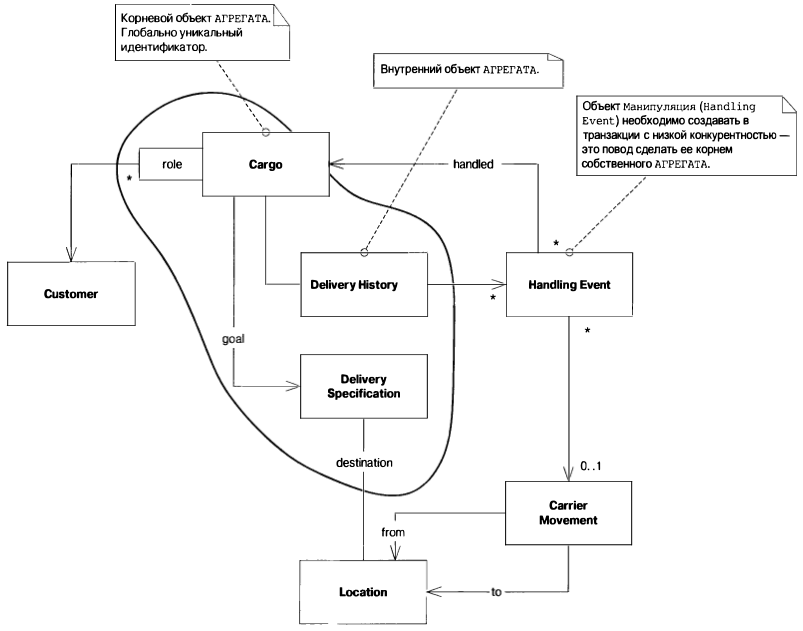
\includegraphics[width=0.7\textwidth]{cargoAggregates.png}
\end{center}

Последнее, что надо решить --- какие репозитории будут использоваться в системе. Надо, очевидно, умет находить груз по Клиенту, Клиента по имени и по грузу, Location по имени города или по идентификатору порта, Перевозку (опять-таки, приплыл корабль --- нашли его в базе и запросили все Handling Event-ы, с ним связанные). Handling Event-у репозиторий пока не нужен, потому что его всегда можно найти по истории Груза, а требований, касающихся отслеживания грузов, которые перевозит корабль, пока нет. Поэтому пока получилось как-то так:

\begin{center}
    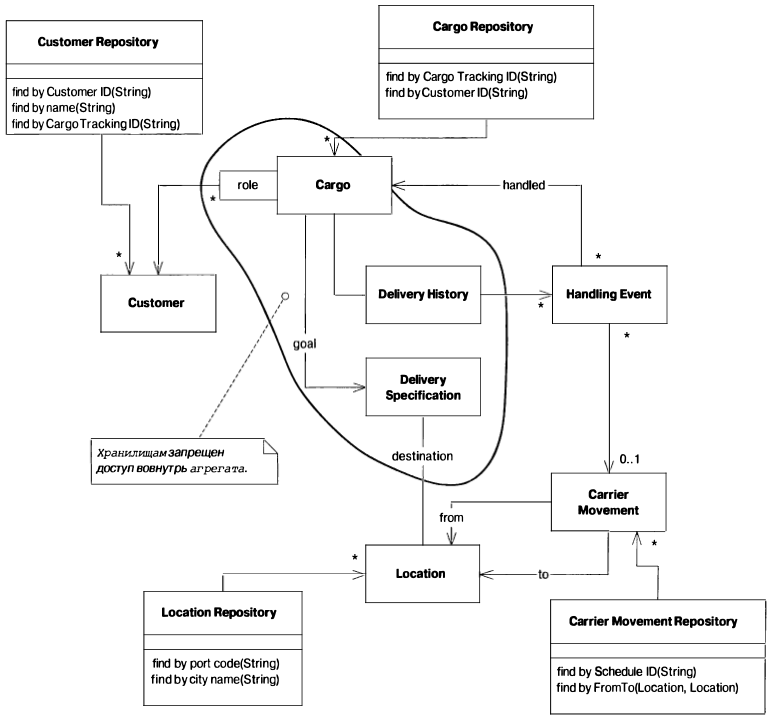
\includegraphics[width=0.7\textwidth]{cargoRepositories.png}
\end{center}

Опробуем получившуюся модель, пройдёсь по одному из случаев использования --- добавлению события манипуляции с грузом сотрудником логистической компании в порту. Поскольку мы решили не делать репозиторий для Handling Event-ов и ассоциация от Перевозки к Handling Event-у у нас однонаправленная, то получится как-то так:

\begin{center}
    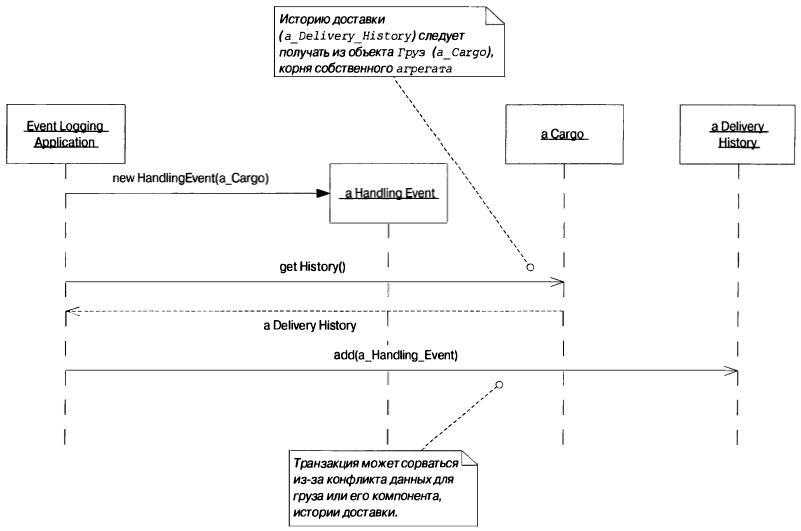
\includegraphics[width=0.7\textwidth]{cargoAddEvent.png}
\end{center}

Получилось не очень удобно, запрос делается весьма окольными путями, да ещё и блокирует половину базы данных в процессе (нам требуется весь агрегат ``Груз'', чтобы добавить событие в его историю).

Поэтому необходим рефакторинг, который исправил бы последствия допущенной нами ошибки. Давайте всё-таки сделаем Handling Event-ам свой репозиторий, и не будем ссылаться на Handling Event из Delivery History напрямую. Ссылку теперь, раз есть репозиторий, можно заменить на запрос к базе:

\begin{center}
    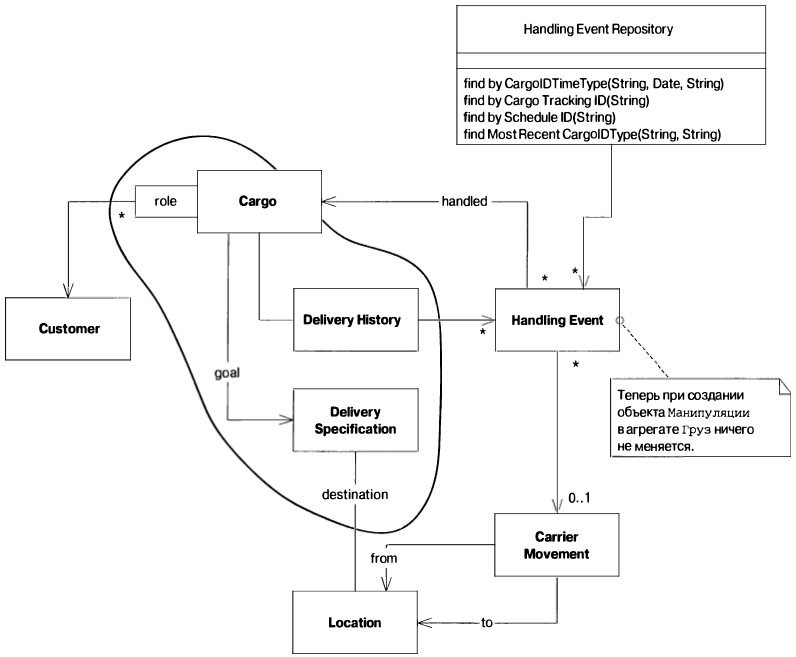
\includegraphics[width=0.7\textwidth]{cargoRefactored.png}
\end{center}

Стало лучше, теперь при добавлении нового события в агрегате ``Груз'' ничего не меняется. В концептуальной модели ассоциация между Delivery History и Handling Event есть, но в коде она реализуется как запрос к репозиторию.

\section{Разбиение по модулям}

Пример с грузоперевозками понадобится нам ещё для того, чтобы обсудить важный принцип DDD о том, что разбиение на модули должно выполняться не механически (например, по типам), а семантически, с учётом требований предметной области. Представим себе, что проектирование системы грузоперевозок дошло до стадии, когда объектов стало слишком много и потребовались модули для декомпозиции системы. Можно сделать плохо, разделив все классы по модулям на основании их типов --- сущности, значения или службы:

\begin{center}
    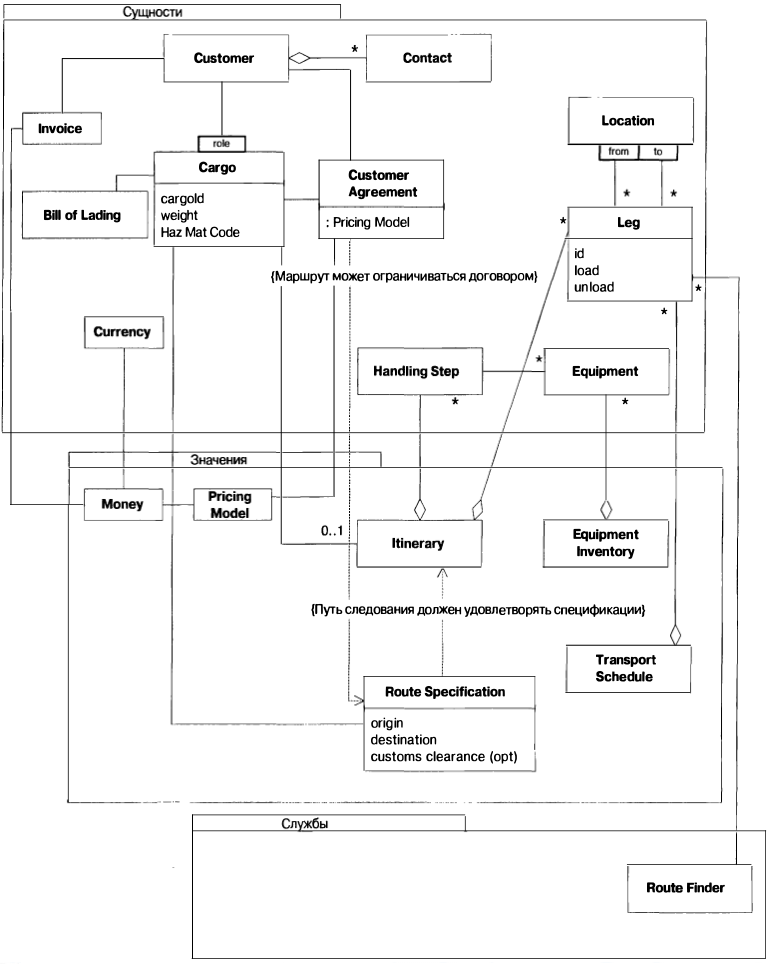
\includegraphics[width=0.9\textwidth]{cargoModulesBad.png}
\end{center}

А можно --- хорошо, в соответствии с единым языком. Программа работает с Клиентом, выполняя Доставку, за что берёт с него Деньги:

\begin{center}
    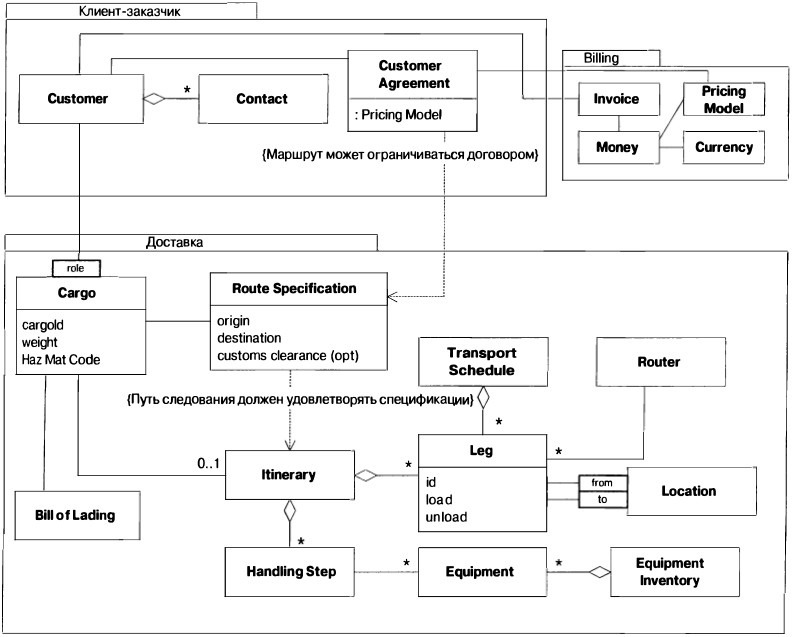
\includegraphics[width=0.8\textwidth]{cargoModulesGood.png}
\end{center}

Как видим, при таком разделении сопряжение и связность тоже стали лучше. На самом деле, это не всегда так, иногда чисто механическая гонка за low coupling и high cohesion ухудшает модель, а не улучшает её. Главное в модели --- это не метрики, а её объясняющая способность.

\section{Моделирование ограничений}

Отвлечёмся от примера про систему грузоперевозок и рассмотрим такой важный момент проектирования, как моделирование и реализацию ограничений на состояние системы. Как мы увидим, ограничения могут привести к внезапному появлению новых объектов в модели, которых как будто не было в предметной области. 

Рассмотрим простой пример --- ведро. В него можно налить. Но не больше, чем в него помещается. Такие дела.

\begin{center}
    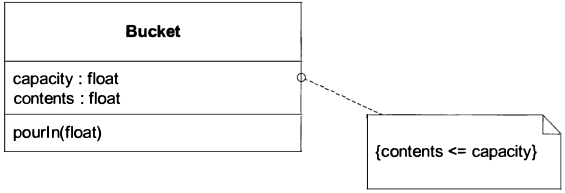
\includegraphics[width=0.5\textwidth]{bucket.png}
\end{center}

Как это можно было бы реализовать на Java:

\begin{minted}{java}
class Bucket {
    private float capacity;
    private float contents;

    public void pourIn(float addedVolume) {
        if (contents + addedVolume > capacity) {
            contents = capacity;
        } else {
            contents = contents + addedVolume;
    }
}
\end{minted}

На самом деле, так себе --- код проверки ограничения смешан с кодом, делающим полезную работу, и несмотря на то, что тут и так всё просто, можно сделать лучше, вынеся проверку ограничения явно:

\begin{minted}{java}
class Bucket {
    private float capacity;
    private float contents;

    public void pourIn(float addedVolume) {
        float volumePresent = contents + addedVolume;
        contents = constrainedToCapacity(volumePresent);
    }

    private float constrainedToCapacity(float volumePlacedIn) {
        if (volumePlacedIn > capacity) return capacity;
        return volumePlacedIn;
    }
} 
\end{minted}

Теперь у нас есть метод, у которого есть говорящее имя, по которому сразу понятно, что происходит, и ограничение уже не потерять.

Однако более сложным ограничениям и в отдельном методе становится тесно. Тогда имеет смысл создать отдельный класс, работа которого будет состоять в проверке объекта на соответствие некоторому ограничению. Как правило, такой класс содержит в себе булевый метод, который говорит, удовлетворяет объект спецификации или нет:

\begin{center}
    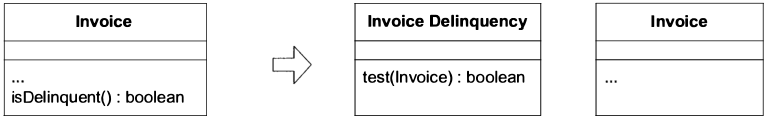
\includegraphics[width=0.8\textwidth]{specification.png}
\end{center}

Особенно хорошо то, что спецификация хорошо работает с паттерном ``Компоновщик'', что позволяет создавать сложные спецификации, комбинируя более простые:

\begin{center}
    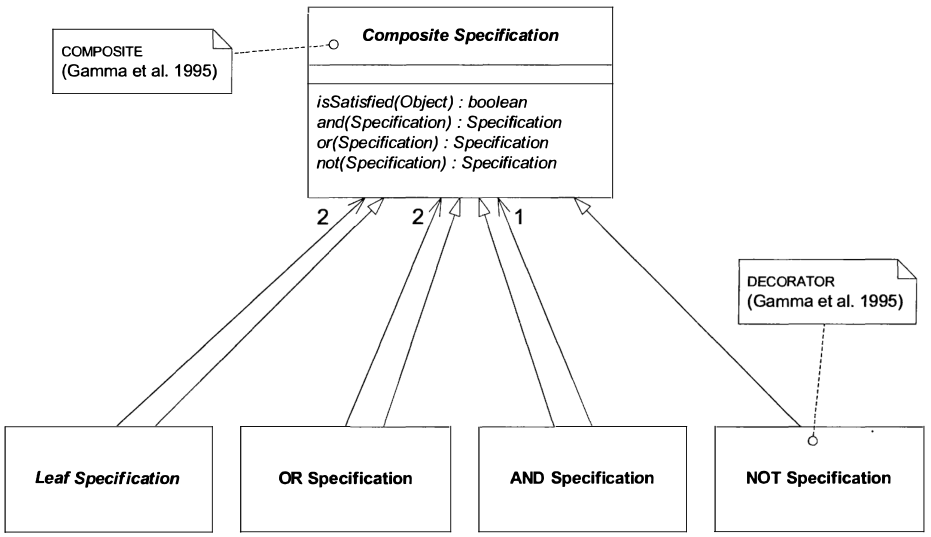
\includegraphics[width=0.8\textwidth]{compositeSpecifications.png}
\end{center}

Спецификация полезна не только для проверки ограничений как большой и страшный assert, но, и прежде всего, как инструмент передачи требований при выборке объекта или при его конструировании в фабрике. Спецификация позволяет сказать, например, ``Хочу граф, однонаправленный, где, скорее всего, будет примерно столько же вершин, сколько и ребёр'', и по этой спецификации фабрика может выбрать наиболее подходящую реализацию графа. В более распространённом для информационных систем случаев спецификация может представлять собой что-то вроде дерева разбора оператора SQL, скорее всего, сильно упрощённого, чтобы ей всё ещё удобно было пользоваться.

Небольшой пример того, как это выглядит в коде. Положим, у нас есть склад химикатов, где химикаты хранятся в бочках (Drum) внутри контейнеров. Химикаты бывают обычные, легко испаряющиеся и взрывоопасные, соответственно, и хранить их надо либо в обычных контейнерах, либо в контейнерах с вентиляцией, либо в бронированных контейнерах. Обычные химикаты можно хранить где угодно, но мы хотим добиться того, чтобы место в контейнерах использовалось наиболее эффективно. Модель предметной области могла бы быть такой:

\begin{center}
    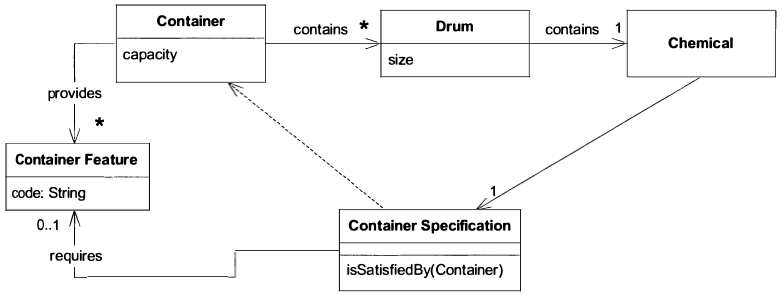
\includegraphics[width=0.8\textwidth]{chemicalsStructure.png}
\end{center}

Каждый контейнер обеспечивает сколько-то характеристик (container feature), и требования химиката касательно условий хранения можно записать как спецификацию, которой может удовлетворять контейнер. У каждого химиката есть ссылка на спецификацию, спецификация может ссылаться на характеристику контейнера и проверять контейнер на то, обладает он характеристикой или нет. В коде это выглядит очень просто:

\begin{minted}{java}
public class ContainerSpecification {
    private ContainerFeature requiredFeature;

    public ContainerSpecification(ContainerFeature required) {
        requiredFeature = required;
    }

    boolean isSatisfiedBy(Container aContainer) {
        return aContainer.getFeatures().contains(requiredFeature);
    }
}
\end{minted}

Ну и в классе Контейнер можно воспользоваться спецификацией, чтобы проверить, правильно ли он заполнен:

\begin{minted}{java}
boolean isSafelyPacked() {
    Iterator it = contents.iterator();
    while (it.hasNext()) {
        Drum drum = (Drum) it.next() ;
        if (!drum.containerSpecification().isSatisfiedBy(this))
            return false ;
    }
    return true;
}
\end{minted}

Как видим, получилось довольно объектно-ориентированно и аккуратно.

\section{Гибкая архитектура}

Ну и последнее, про что следует рассказать, говоря про ``тактические'' аспекты DDD --- это приёмы обеспечения ``гибкости'' архитектуры, то есть набор несложных правил кодирования, которые сделают рефакторинг (в том числе архитектурный) гораздо более безболезненным.

Рассмотрим для примера задачу расчёта смешения красок в строительном магазине. Есть краска, характеризующаяся своим объёмом и цветом (в шкале RGB), надо по данным двум краскам посчитать, какой краской будет результат их слияния. Вот исходное состояние нашей системы:

\begin{center}
    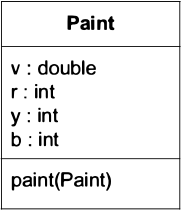
\includegraphics[width=0.15\textwidth]{originalPaint.png}
\end{center}

\begin{minted}{java}
public void paint (Paint paint) {
    v = v + paint.getV();  // После смешивания объем суммируется
// Опущено много строк сложного расчета смешивания цветов,
// который заканчивается присваиванием новых значений
// компонентов r (красного), b (синего) и y (желтого).
}
\end{minted}

Первое правило заключается в том, что, гм, надо делать хорошо и не надо делать плохо. Более конкретно, имена, используемые в программе, должны соответствовать предметной области и объяснять происходящее в коде:

\begin{center}
    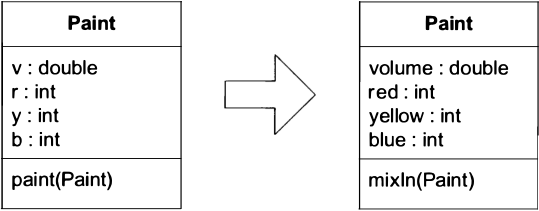
\includegraphics[width=0.4\textwidth] {informativeInterfaceForPaint.png}
\end{center}

\begin{minted}{java}
public void testPaint() {
    // Начинаем с чистой желтой краски объемом = 100
    Paint ourPaint = new Paint(100.0, 0, 50, 0);
    // Берем чистую синюю краску объемом = 100
    Paint bluе = new Paint(100.0, 0, 0, 50);
    // Примешиваем синюю краску к желтой
    ourPaint.mixIn(blue); 
    // Должно получиться 200.0 единиц зеленой краски
    assertEquals(200.0, ourPaint.getVolume(), 0.01);
    assertEquals(25, ourPaint.getBlue());
    assertEquals(25, ourPaint.getYellow());
    assertEquals(0, ourPaint.getRed());
}
\end{minted}

Однако более интересное правило --- правило избегания побочных эффектов и активного использования немутабельных объектов. Проблема:

\begin{center}
    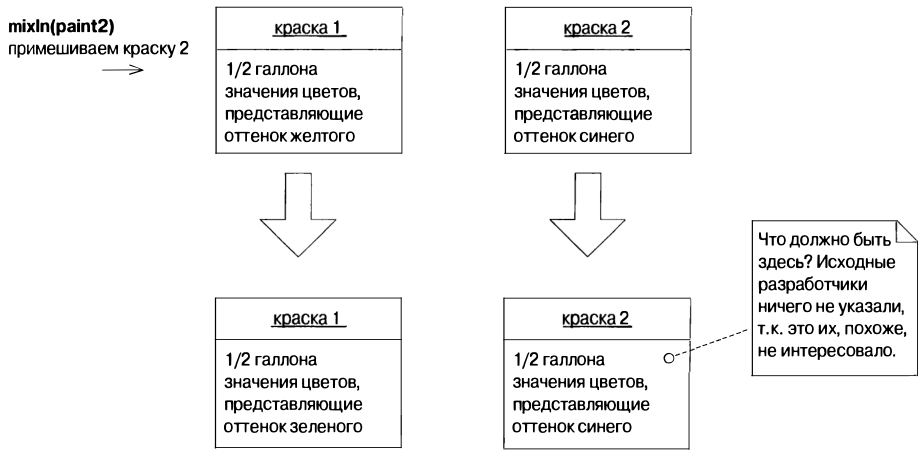
\includegraphics[width=0.7\textwidth]{mixinSideEffects.png}
\end{center}

Программа работает правильно, просто она непонятна. А мы знаем, что хорошая модель (и, следовательно, хорошее её выражение в коде) должно прежде всего объяснять. Существующая модель ничего не говорит о том, что будет со второй краской, у вдумчивого разработчика появляются вопросы, а это как раз то, чего модель должна помогать избегать --- она должна отвечать на вопросы, а не ставить их.

Поэтому посмотрим на смешивание красок по-другому. Выделим сущность ``цвет'', и сделаем краску сущностью, которая обладает этим самым цветом и объёмом. Ещё сделаем наблюдение, что цвет результата на самом деле зависит не от объёма, а от процентного соотношения объёмов смешиваемых цветов. Получаем вот такую модель:

\begin{center}
    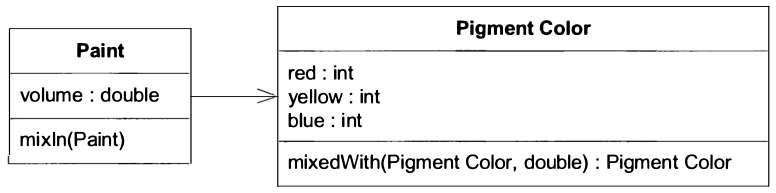
\includegraphics[width=0.8\textwidth]{pigmentColor.png}
\end{center}

И вот такой код:

\begin{minted}{java}
public class PigmentColor {
    public PigmentColor mixedWith(PigmentColor other, double ratio) {
        // Много строк сложного расчета смешивания цветов.
        // в результате создается новый объект PigmentColor
        // с новыми пропорциями красного, синего и желтого.
    }
}

public class Paint {
    public void mixIn(Paint other) {
        volume = volume + other.getVolume();
        double ratio = other.getVolume() / volume;
        pigmentColor = pigmentColor.mixedWith(other.pigmentColor(), ratio);
    }
}
\end{minted}

Теперь вместо того, чтобы думать, что произойдёт с примешиваемой краской, мы оперируем смешиванием цветов, результатом которого станет новый цвет, и оба старых цвета гарантированно не изменятся:

\begin{center}
    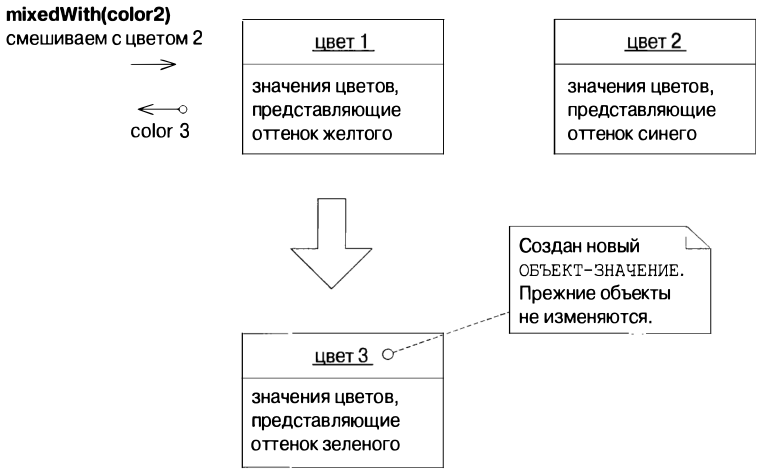
\includegraphics[width=0.8\textwidth]{pigmentColorValueObject.png}
\end{center}

Осталось только разобраться с объёмами, в самой краске, потому как цвет про объём теперь ничего не знает.

Сейчас получается довольно-таки странно:

Постусловие для mixIn():
{\color{blue}
\begin{verbatim}
После pl.mixIn(p2):
    pl.volume увеличивается на объем p2.volume
    p2.volume не изменяется
\end{verbatim} }
И инвариант:
{\color{blue}
\begin{verbatim}
Общий объем краски не должен измениться от смешивания
\end{verbatim} }

Пока что модель вообще противоречива, её объясняющая способность нулевая. Зарефакторим её. Разделим понятия ``краска'' и ``смесь красок'', так что смесь можно формирвоать только из заранее известного набора базовых красок, которые берутся с заданным объёмом. И никакого смешения красок каждый раз на самом деле не происходит, смесь просто хранит в себе список базовых красок с объёмами, и при необходимости вычисляет получившийся цвет. Получилось как-то так:

\begin{center}
    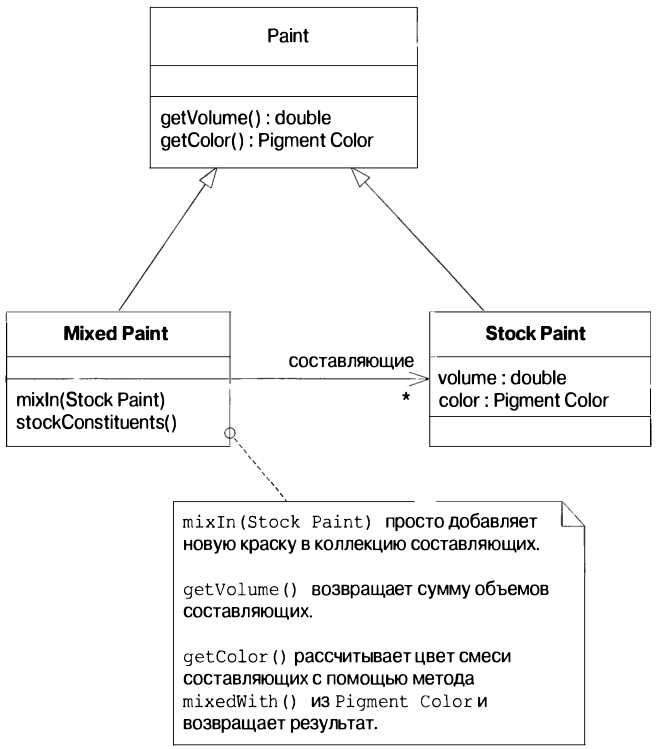
\includegraphics[width=0.6\textwidth]{stockPaints.png}
\end{center}

Понятно, что это не единственное возможное решение, но оно вполне работоспособно, убирает возможные противоречия из модели и даже соответствует предметной области --- в строительном магазине не смешивают обычно уже смешанные краски.

А выявить и решить проблему нам на самом деле помогло явное выписывание предусловий и инвариантов. Хорошо их выписывать не просто текстом, а в коде, с использованием операторов (или функций) assert, которые в том или ином виде присутствуют в любом нормальном языке. Это с одной стороны дополнительный текст, объясняющий, что происходит в модели, с другой стороны, работающий механизм, который поможет сразу выявить проблемы. Чем больше assert-ов --- тем лучше.

\end{document}